% Copyright 2005-2016 Airbus-EDF-IMACS-Phimeca
% Permission is granted to copy, distribute and/or modify this document
% under the terms of the GNU Free Documentation License, Version 1.2
% or any later version published by the Free Software Foundation;
% with no Invariant Sections, no Front-Cover Texts, and no Back-Cover
% Texts.  A copy of the license is included in the section entitled "GNU
% Free Documentation License".
\renewcommand{\nomfichier}{docref_Cprime212_Pearson}
\renewcommand{\titrefiche}{Uncertainty ranking using Pearson's correlation}

\Header

\MathematicalDescription{
  \underline{\textbf{Goal}} \vspace{2mm}

  This method deals with analysing the influence the random vector $\vect{X} = \left( X^1,\ldots,X^{n_X} \right)$ has on a random variable $Y^j$ which is being studied for uncertainty. Here we attempt to measure linear relationships that exist between $Y^j$ and the different components $X^i$. \vspace{2mm}

  \underline{\textbf{Principle}} \vspace{2mm}

  Pearson's correlation coefficient $\rho_{Y^j,X^i}$, defined in  \otref{docref_B231_Pearson}{Pearson's Coefficient}, measures the strength of a linear relation between two random variables $Y^j$ and $X^i$. If we have a sample made up of  $N$ pairs $(y^j_1,x^i_1)$, $(y^j_2,x^i_2)$, \ldots, $(y^j_N,x^i_N)$, we can obtain $\widehat{\rho}_{Y^j,X^i}$ an estimation of Pearson's coefficient. The hierarchical ordering of Pearson's coefficients is of interest in the case where the relationship between $Y^j$ and $n_X$ variables $\left\{ X^1,\ldots,X^{n_X} \right\}$ is close to being a linear relation:
  \begin{align*}
    Y^j \simeq a_0 + \sum_{i=1}^{n_X} a_i X^i
  \end{align*}
  To obtain an indication of the role played by each $X^i$ in the dispersion of $Y^j$, the idea is to estimate Pearson's correlation coefficient  $\widehat{\rho}_{X^i,Y^j}$ for each $i$. One can then order the $n_X$ variables $X^1,\ldots, X^{n_X}$ taking absolute values of the correlation coefficients: the higher the value of  $\left| \widehat{\rho}_{X^i,Y^j} \right|$  the greater the impact the variable $X^i$ has on the dispersion of $Y^j$.

  \begin{center}
    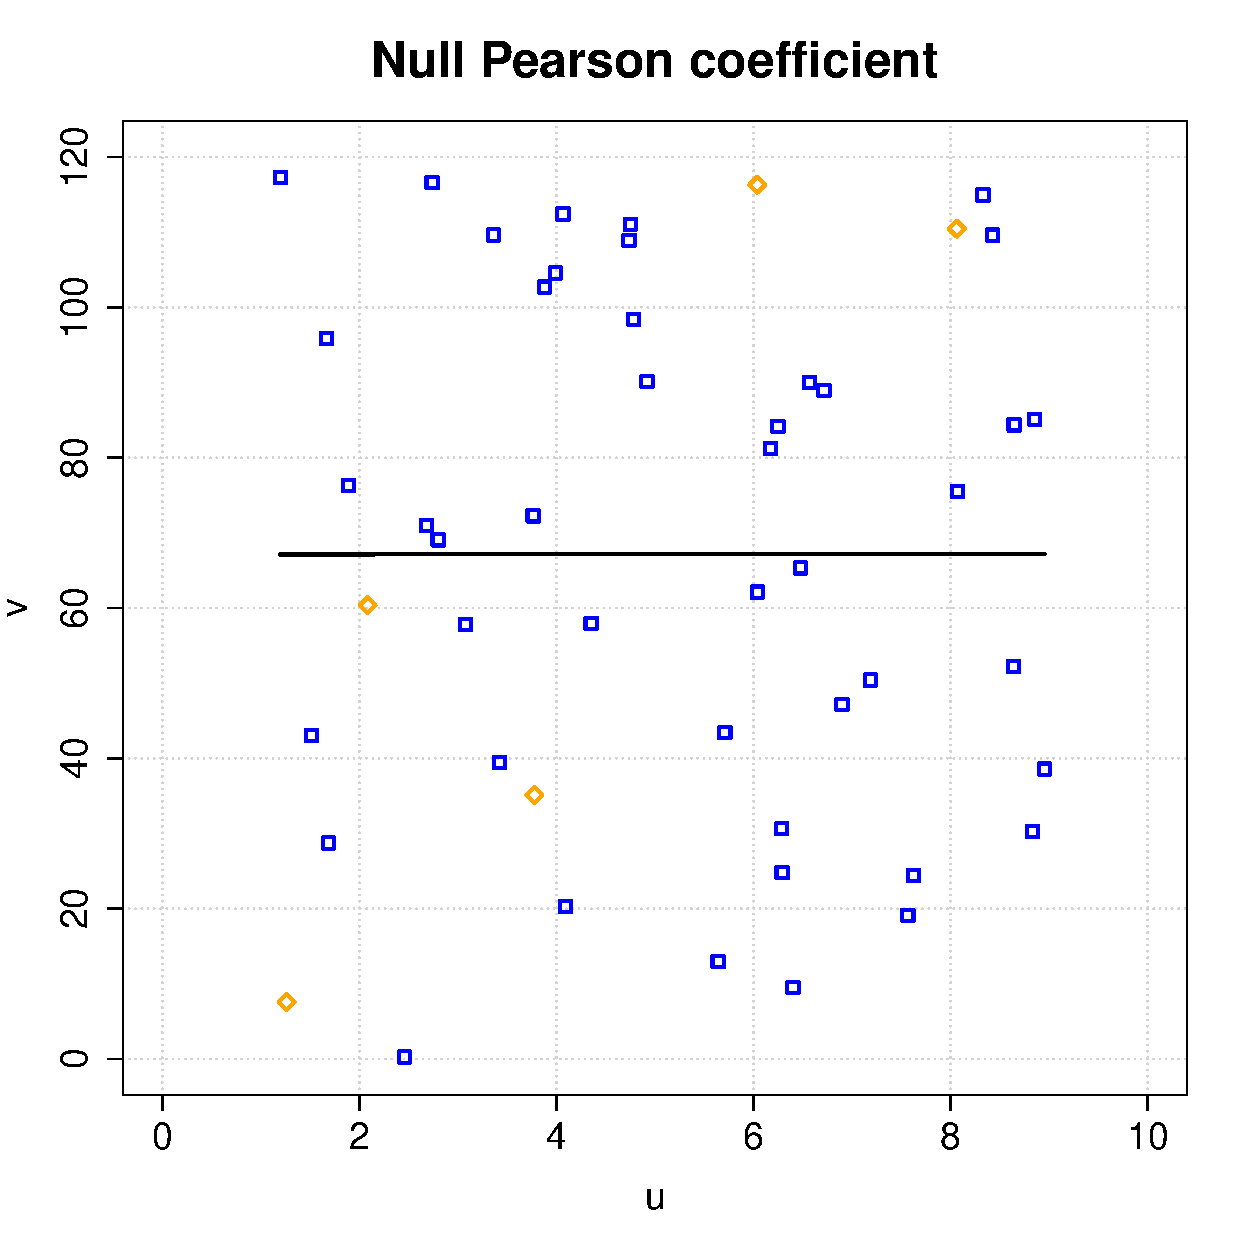
\includegraphics[width=0.5\textwidth]{Figures/pearson3.pdf}
  \end{center}
}
{
  -
}

\Methodology{
  After a propagation of uncertainty (step C) using \otref{docref_C221_MonteCarloStd}{Standard Monte Carlo} simulation, a hierarchy of sources of uncertainty can be obtained using Pearson's correlation coefficients. In fact, the $N$ simulations enable the pairs  $(y^j_1, x^i_1)$, $(y^j_2, x^i_2)$,\ldots, $(y^j_N, x^i_N)$ to be generated, where:
  \begin{itemize}
  \item $\underline{X} = \left\{ X^1,\ldots,X^n \right\}$ describes the input vector specified in  step A "Specifying Criteria and the Case Study",
  \item $Y^j$ describes a variable of interest or output variable defined in the same step.
  \end{itemize}

  The results produced as output of this method are the estimated Pearson's correlation coefficients $\widehat{\rho}_{X^i,Y^j}$ that the user may use, taking absolute values, to order the variables $X^i$ hierarchically.
}
{
  This method of uncertainty ranking is particularly useful:
  \begin{itemize}
  \item when the study of uncertainty deals with the central dispersion of the variable of interest $Y^j$ and not with its extreme values,
  \item when the relationships between $Y^j$ and each of the components of $\underline{X}$ are close to linear relationships (so that Pearson's correlation coefficient can be interpreted),
  \item when this linear relationship is close to  $Y^j = a_0 + \sum_{i=1}^{n_X} a_i X^i$ (i.e. no product terms of the type $X^i X^j$), and when the components of vector $\underline{X}$ are statistically independent.  If this is not the case, $\left| \widehat{\rho}_{X^i,Y^j} \right|$  reflects not only the influence of $X^i$ on $Y^j$ but equally the influence of  other variables $X^j$ related to $X^i$ (e.g. an unimportant variable $X^i$ could have a strong coefficient for the correlation with $Y^j$ only because it is related -- statistically or by a product term -- to another variable $X^j$ which has enormous impact on $Y^j$).
  \end{itemize}

  Readers interested in other methods of uncertainty ranking that can be applied after Monte-Carlo simulation when the assumptions of linearity and/or independence are violated are also referred to \otref{docref_Cprime212_Spearman}{Uncertainty ranking using Spearman}, \otref{docref_Cprime212_SRC}{Hierarchical Ordering using SRC}, \otref{docref_Cprime212_PCC}{Uncertainty ranking with Pearson's Partial Correlation Coefficients} and \otref{docref_Cprime212_PRCC}{Uncertainty ranking using Spearman's Partial Correlation Coefficients}.

  The following references provide an interesting bibliographic starting point to further study of the method described here:
  \begin{itemize}
  \item Saltelli, A., Chan, K., Scott, M. (2000). "Sensitivity Analysis", John Wiley \& Sons publishers, Probability and Statistics series
  \item J.C. Helton, F.J. Davis (2003). "Latin Hypercube sampling and the propagation of uncertainty analyses of complex systems". Reliability Engineering and System Safety 81, p.23-69
  \item J.P.C. Kleijnen, J.C. Helton (1999). "Statistical analyses of scatterplots to identify factors in large-scale simulations, part 1 : review and comparison of techniques". Reliability Engineering and System Safety 65, p.147-185
  \end{itemize}
}
